\chapter{From Path Integrals to Propagators and Vertices}

Before turning to the inventory of particles and their interactions, it is worth making the central construction clear. A Lagrangian does more than encode classical field equations. Through the path integral it also supplies amplitudes for particles to propagate, split, join, and scatter. This is the most direct route from quantum field theory to Feynman diagrams.

\section{Least Action for Particles and Fields}

Feynman's path integral is the quantum counterpart of the principle of least action. Begin with an ordinary Newtonian particle, whose Lagrangian depends on its coordinates and velocities,
\begin{equation}
\mathcal{L}=\mathcal{L}(x,\dot{x}),
\end{equation}
and the action assigned to a trajectory is
\begin{equation}
S[x]=\int \mathcal{L}(x,\dot{x})\,dt.
\end{equation}
Every candidate trajectory from one spacetime point to another has an action, whether or not it satisfies Newton's equations. The classical trajectory is distinguished by stationary action. In the traditional ``least-action'' language it minimizes the action, although stationary is the more general statement. The stationarity condition gives the classical differential equations of motion.

\begin{figure}[htbp]
\centering

\includegraphics[width=0.72\textwidth]{lecture_10_figure_02.png}
\caption{Action integral for a particle trajectory.}
\lectureframe{00:02:14}
\end{figure}

The same structure applies to a classical field. Write all the fields generically as \(\phi\). A local field Lagrangian density may depend on the fields and on both their spatial and temporal derivatives:
\begin{equation}
\mathcal{L}
=\mathcal{L}\!\left(\phi,\frac{\partial\phi}{\partial x^\mu}\right)
=\mathcal{L}(\phi,\partial_\mu\phi).
\end{equation}
Relativity requires \(\mathcal{L}\) to transform as a Lorentz scalar. Subject to that requirement, scalar combinations built from fields and their derivatives furnish the possible terms in the Lagrangian.

\begin{figure}[htbp]
\centering

\includegraphics[width=0.62\textwidth]{lecture_10_figure_03.png}
\caption{Dependence of the field Lagrangian on the field and its spacetime derivatives.}
\lectureframe{00:04:09}
\end{figure}

For a field, the action is integrated over a region of spacetime:
\begin{equation}
S[\phi]=\int_{\Omega} d^4x\,\mathcal{L}(\phi,\partial_\mu\phi),
\qquad
d^4x=dt\,dx\,dy\,dz.
\end{equation}
The particle action is an integral over time along a path. The field action is the integrated Lagrangian density throughout a spacetime region.

The analog of fixing the endpoints of a particle path is to prescribe the complete field configuration on an initial time slice and on a final time slice. If the initial field is \(\phi_{\mathrm{i}}(\mathbf{x})\) and the final field is \(\phi_{\mathrm{f}}(\mathbf{x})\), an interpolating field fills the whole slab between them. When the boundary data admit a classical interpolating solution, that solution is a stationary point of the action with the boundary configurations held fixed.
\editorialnote{Arbitrary complete field configurations on two time slices need not admit a classical solution. The stationary-action statement is therefore restricted to boundary data for which an interpolating solution exists.}

The geometry is the field-theory counterpart of a particle path.\footnote{The spacetime slab is reconstructed from the diagram at approximately 00:04:29.}
\begin{figure}[htbp]
\centering
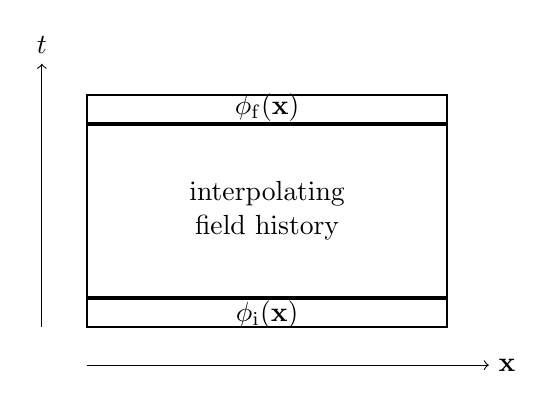
\begin{tikzpicture}[scale=0.88]
\draw[->] (-0.65,0) -- (-0.65,3.8) node[above] {$t$};
\draw[->] (0,-0.55) -- (5.8,-0.55) node[right] {$\mathbf{x}$};
\draw[thick] (0,0) rectangle (5.2,3.35);
\draw[very thick] (0,0.42) -- (5.2,0.42);
\draw[very thick] (0,2.93) -- (5.2,2.93);
\node at (2.6,0.18) {$\phi_{\mathrm{i}}(\mathbf{x})$};
\node at (2.6,3.17) {$\phi_{\mathrm{f}}(\mathbf{x})$};
\node[align=center] at (2.6,1.68) {interpolating\\field history};
\end{tikzpicture}
\caption{Initial and final field configurations bounding a spacetime region.}
\end{figure}

\begin{classroomqa}
\lecturetimestamp{00:07:34}
\audiencequestion{Can a field return to the same value?}
\lecturerresponse{Yes. There is no obstruction to a field returning to an earlier value, just as there is no obstruction to a particle coordinate returning to an earlier position.}
\end{classroomqa}

\begin{classroomqa}
\lecturetimestamp{00:07:46}
\audiencequestion{Why speak of spacetime events or a trajectory when the boundary data are field values?}
\lecturerresponse{The particle trajectory is replaced by a field history. Each endpoint in field space is the whole field on a chosen time slice, and a history specifies the field at every point in the spacetime region between the two slices.}
\end{classroomqa}

Requiring stationary action for the interpolating field produces partial differential equations. Depending on the fields and the Lagrangian, these include equations such as Maxwell's equations and, for a gravitational action, Einstein's equations. The detailed variational derivation is not needed here; the important sequence is
\begin{equation}
\mathcal{L}
\longrightarrow
S[\phi]
\longrightarrow
\text{classical field equations}.
\end{equation}

\section{Feynman's Sum over Particle Paths}

Quantum mechanics replaces the question of which trajectory occurs by a question about amplitudes. Imagine injecting a particle at \((x,t)\), closing one's eyes for a while, and then turning on a detector at \((x',t')\). The amplitude
\begin{equation}
\mathcal{A}(x,t;x',t')
\end{equation}
is a complex number. Its magnitude squared is the probability:
\begin{equation}
\begin{aligned}
P(x,t;x',t')
&=\left|\mathcal{A}(x,t;x',t')\right|^2\\
&=\mathcal{A}(x,t;x',t')
\mathcal{A}(x,t;x',t')^*.
\end{aligned}
\end{equation}

Feynman's rule assigns an action to every candidate path and associates with it the phase
\begin{equation}
\exp\!\left(-\frac{i}{\hbar}S[x]\right)
=
\exp\!\left[-\frac{i}{\hbar}\int \mathcal{L}(x,\dot{x})\,dt\right].
\end{equation}

\begin{figure}[htbp]
\centering

\includegraphics[width=0.70\textwidth]{lecture_10_figure_04.png}
\caption{Complex phase associated with a particle path.}
\lectureframe{00:11:52}
\end{figure}

The factor of \(\hbar\) is required to make the exponent dimensionless.\footnote{At 00:11:52 the board reads naturally as \(e^{-i\int\mathcal{L}\,dt}\); the factor of \(\hbar\) is supplied in speech at 00:12:02.} The transition amplitude is the sum of these phases over every possible path connecting the endpoints:
\begin{equation}
\mathcal{A}(x,t;x',t')
=
\sum_{\substack{\text{paths }x(\tau)\\(x,t)\rightarrow(x',t')}}
\exp\!\left(-\frac{i}{\hbar}S[x]\right).
\end{equation}
Here ``possible path'' does not mean a solution of Newton's equations. It means any path included in the sum. In nonrelativistic quantum mechanics the paths progress forward in time rather than looping backward. Planck's constant has the dimensions of action, so \(S/\hbar\) is dimensionless.

The exponential is natural because amplitudes for successive small steps multiply. If a path is divided into consecutive pieces, the action adds,
\begin{equation}
S=S_1+S_2+\cdots,
\end{equation}
while the phases multiply:
\begin{equation}
e^{-iS/\hbar}
=e^{-iS_1/\hbar}e^{-iS_2/\hbar}\cdots.
\end{equation}
The factor \(i\) is not a bookkeeping device; it is part of the quantum-mechanical rule.

\begin{classroomqa}
\lecturetimestamp{00:13:27}
\audiencequestion{Is the exponential connected with multiplying the amplitudes for successive small steps?}
\lecturerresponse{Yes. Successive step amplitudes multiply, while the corresponding pieces of the action add.}
\end{classroomqa}

\begin{classroomqa}
\lecturetimestamp{00:13:49}
\audiencequestion{Is the sum over paths itself the probability?}
\lecturerresponse{No. The path sum is a generally complex probability amplitude. Multiplying it by its complex conjugate gives the probability.}
\end{classroomqa}

\section{The Sum over Field Histories}

The same formulation extends to quantum field theory, although the construction here will remain deliberately nonrigorous. Begin with an initial field configuration \(\phi(\mathbf{x})\) and a separately specified final configuration \(\phi'(\mathbf{x})\). These are complete functions of space, not values at two isolated points.

One may imagine an idealized apparatus that prepares the field at every spatial point, lets the system evolve, and later measures the field at every point. Such an apparatus is not realistic, but it defines the conceptual question cleanly: what is the amplitude to pass from the initial complete field configuration to the final one?

Every imaginable interpolating field history contributes. For each history, evaluate
\begin{equation}
S[\phi]=\int d^4x\,\mathcal{L}(\phi,\partial_\mu\phi)
\end{equation}
and attach the corresponding phase. Schematically,
\begin{equation}
\mathcal{A}\!\left[\phi(\mathbf{x})\rightarrow\phi'(\mathbf{x})\right]
=
\sum_{\substack{\text{field histories}\\
\phi_{\mathrm{i}}=\phi,\;\phi_{\mathrm{f}}=\phi'}}
\exp\!\left(-\frac{i}{\hbar}S[\phi]\right).
\end{equation}
A history need not solve the classical field equations. It is simply one complete assignment of field values throughout the intervening spacetime region.

\begin{classroomqa}
\lecturetimestamp{00:17:39}
\audiencequestion{There are infinitely many histories, and each phase has magnitude one. How can their sum converge? Are the histories being minimized?}
\lecturerresponse{The histories are summed, not minimized. The terms are phases distributed around the unit circle, so they can cancel one another. This differs from adding infinitely many positive terms bounded away from zero. Oscillatory integrals can converge; the Fourier representation of a delta function is a familiar example. If the phases were distributed uniformly around the circle, their vector sum would vanish. Most histories cancel strongly. Histories near a stationary-action trajectory cancel least because the phase changes least rapidly there, and this is how the classical limit emerges.}
\end{classroomqa}

\editorialnote{A real-time path integral ordinarily requires a convergence prescription. The unit-circle discussion gives the oscillatory-cancellation argument used here, not a general proof of convergence.}

The cancellation can be pictured as a vector sum in the complex plane.\footnote{The unit-circle construction is reconstructed from the board discussion at 00:18:32--00:20:21.}
\begin{figure}[htbp]
\centering
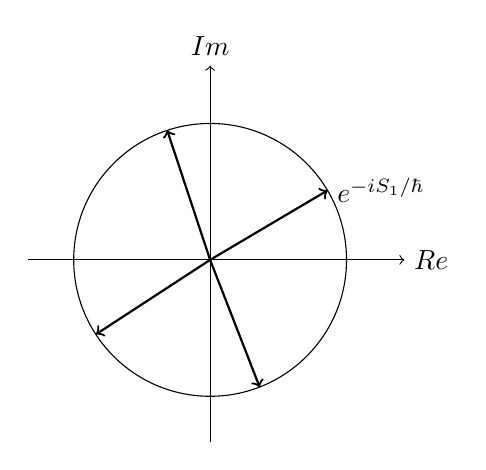
\begin{tikzpicture}[scale=1.05]
\draw[->] (-2.2,0) -- (2.35,0) node[right] {$\operatorname{Re}$};
\draw[->] (0,-2.2) -- (0,2.35) node[above] {$\operatorname{Im}$};
\draw (0,0) circle (1.65);
\draw[thick,->] (0,0) -- (1.42,0.84);
\draw[thick,->] (0,0) -- (-1.38,-0.90);
\draw[thick,->] (0,0) -- (-0.52,1.57);
\draw[thick,->] (0,0) -- (0.60,-1.54);
\node[right] at (1.42,0.84) {$e^{-iS_1/\hbar}$};
\end{tikzpicture}
\caption{Unit-magnitude phases can cancel when their directions differ.}
\end{figure}

Indeed,
\begin{equation}
e^{-iS/\hbar}
=
\cos\!\left(\frac{S}{\hbar}\right)
-i\sin\!\left(\frac{S}{\hbar}\right).
\end{equation}
Each contribution is a unit vector. Contributions pointing in different directions subtract as well as add. Near a stationary point of \(S\), nearby histories have nearly the same phase, so their contributions reinforce one another more effectively. Away from stationary action, the phase varies rapidly and destructive interference dominates.

This path-integral structure underlies essentially all modern quantum field theory. The next practical step will be stated rather than derived. It is an oversimplified route into the calculation, but it makes visible how the same object can be used in two languages.

To calculate a process is to calculate an initial-to-final transition probability. One description specifies an initial field configuration and a final field configuration. The other specifies incoming and outgoing particles, the quanta of one or several fields. These questions look different, but both are calculated from the same field-theory path integral.

\section{A Discrete Spacetime Form}

To give the field-history sum a concrete meaning, divide spacetime into small cells and assign a field value to each cell. The continuum limit is approached by shrinking the cell size, but for now the cells remain finite. This converts the formal sum over functions into a sum over assignments of numbers to lattice cells.

An earlier heuristic uses a product of factors resembling \(1+\mathcal{L}_i\), one for each cell, and then identifies terms describing particle propagation and collision. The construction is central enough to repeat, but the factor must be corrected. The small quantity is not the Lagrangian itself. It is the action contained in a cell.

If a cell has spacetime volume
\begin{equation}
a^4=\Delta t\,\Delta x\,\Delta y\,\Delta z,
\end{equation}
then its action is
\begin{equation}
A_i=\mathcal{L}_i a^4.
\end{equation}
Since the cell is small, \(A_i\) is small. Temporarily suppressing \(\hbar\), the corrected elementary factor is
\begin{equation}
1-iA_i,
\end{equation}
rather than \(1+\mathcal{L}_i\).

For any small \(\epsilon\),
\begin{equation}
1+\epsilon\simeq e^\epsilon,
\end{equation}
because
\begin{equation}
e^\epsilon
=1+\epsilon+\frac{\epsilon^2}{2!}
+\frac{\epsilon^3}{3!}+\cdots.
\end{equation}
Thus, in these temporary units, \(1-iA_i\) approximates \(e^{-iA_i}\) for a sufficiently small cell. It is cleaner to use the exact exponential factor from the beginning.

\begin{classroomqa}
\lecturetimestamp{00:27:57}
\audiencequestion{Does the exponential require a factor of \(\hbar\)?}
\lecturerresponse{Yes. The dimensionless cell factor is \(1-iA_i/\hbar\) to first order, and the exact exponential is \(\exp(-iA_i/\hbar)\). One may later adopt units in which \(\hbar=1\).}
\end{classroomqa}

Restoring \(\hbar\), the corrected intermediate factor and its exponential form are
\begin{equation}
1-\frac{i}{\hbar}A_i
\simeq
\exp\!\left(-\frac{i}{\hbar}A_i\right).
\end{equation}

For a fixed history, replace the spacetime integral by a sum of cell actions:
\begin{equation}
S[\phi]
=\int d^4x\,\mathcal{L}
\;\longrightarrow\;
\sum_i A_i.
\end{equation}
The phase for that history becomes
\begin{equation}
\exp\!\left(-\frac{i}{\hbar}\sum_i A_i\right).
\end{equation}
An exponential of a sum is a product of exponentials:
\begin{equation}
\exp\!\left(-\frac{i}{\hbar}\sum_i A_i\right)
=
\prod_i\exp\!\left(-\frac{i}{\hbar}A_i\right).
\end{equation}
The order of operations matters. First choose one complete history and multiply its cell weights. Only then sum over the different histories.

The lattice also makes the boundary data explicit.\footnote{The checkerboard and its fixed first and last rows are reconstructed from the diagrams at approximately 00:23:54 and 00:30:49.}
\begin{figure}[htbp]
\centering
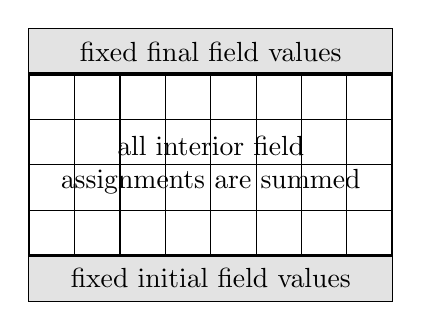
\begin{tikzpicture}[scale=0.72]
\draw[step=0.8,thin] (0,0) grid (6.4,4.8);
\draw[thick] (0,0) rectangle (6.4,4.8);
\fill[gray!22] (0,0) rectangle (6.4,0.8);
\fill[gray!22] (0,4.0) rectangle (6.4,4.8);
\draw[very thick] (0,0.8) -- (6.4,0.8);
\draw[very thick] (0,4.0) -- (6.4,4.0);
\node at (3.2,0.4) {fixed initial field values};
\node at (3.2,4.4) {fixed final field values};
\node[align=center] at (3.2,2.4) {all interior field\\assignments are summed};
\end{tikzpicture}
\caption{Discrete field histories with fixed initial and final lattice rows.}
\end{figure}

The first row specifies the initial field configuration, and the last row specifies the final configuration. Every interior cell is allowed every field value included in the discretization. Thus the transition amplitude takes the schematic form
\begin{equation}
\mathcal{A}\!\left[\phi_{\mathrm{i}}\rightarrow\phi_{\mathrm{f}}\right]
=
\sum_{\{\phi\}_{\mathrm{interior}}}
\prod_i\exp\!\left(-\frac{i}{\hbar}A_i[\phi]\right),
\end{equation}
with the first and last rows held fixed. Equivalently, for each interior assignment one computes the exponential of the total action and then adds that contribution to the contributions from all other assignments.

\section{From Field Configurations to Particle Configurations}

The same transition amplitude may be described in terms of fields or in terms of particles. Instead of fixing the field on the first and last time slices, one may specify an incoming collection of field quanta and an outgoing collection of field quanta, then ask for the amplitude connecting them. The object being evaluated is the same. Only the boundary description has changed.

Quantum fields contain creation and annihilation operators. Products of fields therefore act on particle states by creating, destroying, or moving quanta. This operator reading is what turns the lattice path integral into a set of particle rules.

\begin{classroomqa}
\lecturetimestamp{00:34:11}
\audiencequestion{Are field quanta necessarily identifiable as particles?}
\lecturerresponse{Not always in the conventional sense of separately observable particles. Quarks are quanta of quark fields, for example, but confinement prevents an isolated quark from escaping and being detected by itself. More generally there need not be a one-to-one correspondence between the fields named in a theory and the particle species that appear as conventional observable states. Some field theories do not admit that simple correspondence. If ``particle'' is used broadly to mean an indivisible quantum carrying energy and other quantum numbers, then the distinction can partly become one of terminology.}
\end{classroomqa}

\editorialnote{The source's weak-coupling clause at 00:35:45--00:36:08 is grammatically ambiguous and is left unresolved here. The secure claim is that field labels and conventionally observable particle species need not correspond one-to-one.}

The lattice sum itself still ranges over field values. It is not restricted to configurations that resemble smooth classical solutions.

\begin{classroomqa}
\lecturetimestamp{00:36:44}
\audiencequestion{Must the field histories be continuous, or at least approximately continuous?}
\lecturerresponse{No. On a discrete lattice, neighboring cells simply carry field values, and every assignment is included in the sum. There is no restriction to histories that are approximately continuous. Quantum fields fluctuate strongly; typical histories are not smooth classical fields.}
\end{classroomqa}

The variables assigned independently are the fields at the lattice sites or cells. Their derivatives are obtained from differences between neighboring values.

\begin{classroomqa}
\lecturetimestamp{00:37:56}
\audiencequestion{Are the fields and their derivatives assigned independent values?}
\lecturerresponse{No. Field values are assigned at the sites. A derivative is then reconstructed from the difference between neighboring field values. Different finite-difference conventions are possible, but the derivatives are not additional independent variables.}
\end{classroomqa}

Thus, for lattice spacing \(a\), one may write schematically
\begin{equation}
\partial_\mu\phi(x)
\longrightarrow
\frac{\phi(x+a\hat\mu)-\phi(x)}{a}.
\end{equation}
The field-value axis may itself be divided into small intervals, leaving a countable set of possible values at each site.

\begin{classroomqa}
\lecturetimestamp{00:38:53}
\audiencequestion{What changes when there is more than one field?}
\lecturerresponse{A value of each field is assigned at every site, and the sum runs over all such assignments.}
\end{classroomqa}

A complex-valued field should not be confused with an analytic function of a complex variable. Analyticity is an exceptionally strong smoothness condition. The histories in a field path integral need not obey it and, in general, are not even approximately smooth.

\begin{classroomqa}
\lecturetimestamp{00:39:07}
\audiencequestion{If the fields are complex-valued, must their values satisfy the smoothness conditions obeyed by analytic functions?}
\lecturerresponse{No. Complex-valued does not mean analytic. The theory of analytic functions concerns an extremely smooth and tightly constrained class of functions. The field histories summed here need not be analytic functions of position; typical histories are highly irregular and may be regarded as highly discontinuous in the continuum limit.}
\end{classroomqa}

The resulting computation looks formidable. Even after spacetime and field values have been discretized, there can be an enormous number of assignments to sample.

\begin{classroomqa}
\lecturetimestamp{00:40:04}
\audiencequestion{How does a computer know how many lattice assignments to sample, or when the calculation has converged?}
\lecturerresponse{That question belongs to lattice gauge theory, or more generally lattice quantum field theory. By now it is an effective computational subject. I was involved at the very beginning in setting up the rules for lattice gauge theory, not in the later computer technology. Setting up the rules took about three weeks; developing the technology to compute these things took something like thirty years. Much of the practical wisdom came from statistical mechanics, where partition functions are also obtained by summing over configurations of a lattice---for example, over whether a site in a crystal is occupied. Determining whether enough configurations have been sampled is a technical matter. The experts know---or think they know---when the calculation is under control, and the resulting calculations agree with experiment.}
\end{classroomqa}

The conceptual rules for lattice gauge theory came quickly; the technology required to compute with them took much longer. The checkerboard is not merely an analogy. It is also the starting point of a practical computational method.

\section{Quadratic Terms and Particle Propagation}

Return now to the operator interpretation of the fields. For two neighboring sites \(x\) and \(x'\), the product
\begin{equation}
\phi(x)\phi(x')
\end{equation}
can supply, in an appropriate one-particle matrix element, the annihilation of a particle at one site and its creation at the other. In that particle sector it may therefore be pictured as a one-link hop. This is one reading of the operator product, not its unique meaning.

The terms responsible for such links are the derivative terms. Strictly speaking, they are associated not with one cell but with a neighboring pair. A temporal derivative, for example, becomes
\begin{equation}
\partial_t\phi(t,\mathbf{x})
\longrightarrow
\frac{\phi(t+a,\mathbf{x})-\phi(t,\mathbf{x})}{a},
\end{equation}
and a spatial derivative is treated in the same way along a spatial link.

\begin{classroomqa}
\lecturetimestamp{00:44:39}
\audiencequestion{Do the Lagrangians under discussion contain second derivatives?}
\lecturerresponse{The standard theories being considered here are written with first derivatives. Their lattice versions therefore use first differences between neighboring sites.}
\end{classroomqa}

Squaring a first difference produces both same-site terms and a neighboring cross term:
\begin{align}
\frac{1}{2}\bigl[\phi(x)-\phi(x')\bigr]^2
&=
\frac{1}{2}\phi(x)^2
+\frac{1}{2}\phi(x')^2
-\phi(x)\phi(x').
\end{align}
The cross term can supply motion from one site to the other. The two squares are same-site terms. The quadratic derivative terms are the kinetic terms, and it is their neighboring cross terms that will be used first to build propagation.

To isolate the combinatorics, collect the neighboring products into
\begin{equation}
K=\sum_{\langle x,x'\rangle}\phi(x)\phi(x').
\end{equation}
The corresponding factor in the path-integral weight is written schematically as
\begin{equation}
e^{-iK}.
\end{equation}
\editorialnote{In this schematic lattice factor, powers of the lattice spacing, \(\hbar\), metric signs, normalization constants, and the coefficients of the links are suppressed.}
Its expansion is
\begin{equation}
e^{-iK}
=1-iK-\frac{1}{2!}K^2+\frac{i}{3!}K^3+\cdots,
\end{equation}
or, with the neighboring sums exposed,
\begin{align}
e^{-iK}
={}&1
-i\sum_{\langle x,x'\rangle}\phi(x)\phi(x')
\nonumber\\
&-\frac{1}{2!}
\sum_{\langle x,x'\rangle}
\sum_{\langle y,y'\rangle}
\phi(x)\phi(x')\phi(y)\phi(y')
+\cdots .
\end{align}
Each factor independently selects a neighboring pair.

The particle diagrams obey a no-dangling-end rule. An exposed endpoint is allowed only where the boundary condition explicitly inserts a particle on the initial slice or removes one on the final slice. An isolated link in the interior has unmatched ends and does not represent a complete contribution to the prescribed transition. Internal link ends must join.

Consider first a lattice only two time layers high. If the initial state inserts a particle at \(x\) and the final state removes it at the neighboring point \(x'\), the first-order term can connect the two boundary insertions:
\begin{equation}
x\longrightarrow x',
\qquad
\mathcal{A}_{\text{one link}}\sim -i.
\end{equation}
The coefficient \(-i\) is only the coefficient in this schematic expansion; the suppressed lattice and normalization factors remain understood.

\begin{classroomqa}
\lecturetimestamp{00:52:16}
\audiencequestion{Does the first-order one-link term contribute only when the relevant initial and final sites are adjacent?}
\lecturerresponse{Yes. That term selects one neighboring pair, so it can connect those boundary sites only when they are neighbors. More distant propagation comes from higher-order products.}
\end{classroomqa}

At second order the two factors are independently summed over neighboring pairs:
\begin{equation}
K^2
=
\sum_{\langle x,x'\rangle}
\sum_{\langle y,y'\rangle}
\phi(x)\phi(x')\phi(y)\phi(y').
\end{equation}

\begin{classroomqa}
\lecturetimestamp{00:52:40}
\audiencequestion{Must the second neighboring pair adjoin the pair selected by the first factor?}
\lecturerresponse{No. Each factor independently selects a neighboring pair. The two pairs may share a site, they may be completely separate, or they may even be the same pair. The sum includes every possibility.}
\end{classroomqa}

For one particle propagating across three time layers, the useful second-order selection has a shared intermediate site:
\begin{equation}
\bigl[\phi(x_0)\phi(x_1)\bigr]
\bigl[\phi(x_1)\phi(x_2)\bigr],
\qquad
x_0\longrightarrow x_1\longrightarrow x_2.
\end{equation}
The end of the first link is joined to the beginning of the second. Only the initial endpoint at \(x_0\) and the final endpoint at \(x_2\) remain exposed, so the term contributes to the required one-particle transition. In the schematic exponential its coefficient is
\begin{equation}
-\frac{1}{2!}.
\end{equation}

The selections may instead form separate hops.\footnote{The link diagrams are reconstructed from the sequence at 00:49:18--00:55:12.}
\begin{figure}[htbp]
\centering
\resizebox{\linewidth}{!}{%
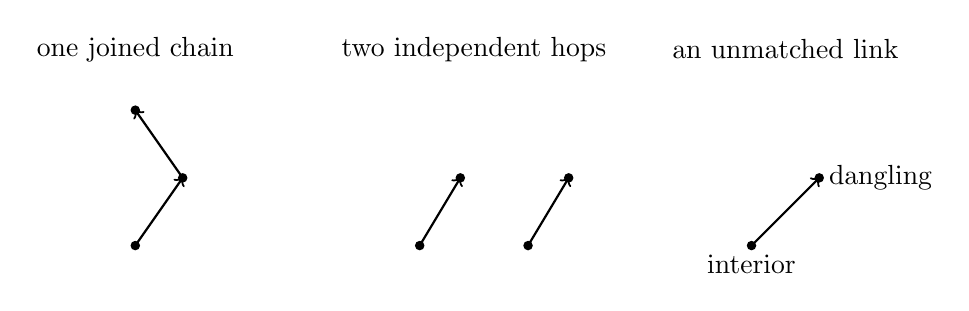
\begin{tikzpicture}[scale=0.86]
\node at (0,2.9) {one joined chain};
\fill (0,0) circle (2pt);
\fill (0.7,1.0) circle (2pt);
\fill (0,2.0) circle (2pt);
\draw[thick,->] (0,0) -- (0.7,1.0);
\draw[thick,->] (0.7,1.0) -- (0,2.0);

\begin{scope}[xshift=4.2cm]
\node at (0.8,2.9) {two independent hops};
\fill (0,0) circle (2pt);
\fill (0.6,1.0) circle (2pt);
\fill (1.6,0) circle (2pt);
\fill (2.2,1.0) circle (2pt);
\draw[thick,->] (0,0) -- (0.6,1.0);
\draw[thick,->] (1.6,0) -- (2.2,1.0);
\end{scope}

\begin{scope}[xshift=9.1cm]
\node at (0.5,2.9) {an unmatched link};
\fill (0,0) circle (2pt);
\fill (1.0,1.0) circle (2pt);
\draw[thick,->] (0,0) -- (1.0,1.0);
\node[below] at (0,0) {interior};
\node[right] at (1.0,1.0) {dangling};
\end{scope}
\end{tikzpicture}%
}
\caption{Joined, independent, and unmatched selections of neighboring links.}
\end{figure}

There can already be more than one route at this order. For a displacement by one temporal and one spatial lattice step, the two orders
\begin{align}
x
&\longrightarrow x+\hat t
\longrightarrow x+\hat t+\hat s,\\
x
&\longrightarrow x+\hat s
\longrightarrow x+\hat s+\hat t
\end{align}
reach the same endpoint.

\begin{classroomqa}
\lecturetimestamp{00:55:53}
\audiencequestion{Is there another two-step path to the same diagonal endpoint?}
\lecturerresponse{Yes. One may take the temporal step first and the spatial step second, or take them in the opposite order. Both routes contribute to the same transition amplitude.}
\end{classroomqa}

There is no reason to stop at two links. The third-order term supplies chains of three neighboring links. A route may advance directly, make a detour, or move away and return before reaching the final point. Still higher orders include longer detours and repeated backtracking. Expanding to arbitrary order therefore produces a contribution for every route assembled from local links. The point-to-point amplitude is the sum of all of them, with coefficients containing the appropriate powers of \(i\) and factorials:
\begin{equation}
\begin{gathered}
\mathcal{A}(x_{\mathrm{in}}\to x_{\mathrm{out}})
=
\sum_{\text{joined lattice routes }r}c_r,
\\
c_r\ \hbox{read from the exponential expansion}.
\end{gathered}
\end{equation}
The coefficients are generally complex, so the resulting amplitude is complex.

Relativistic propagation adds another possibility. A route may run both upward and downward in the time direction, and it may traverse the same link repeatedly.

\begin{classroomqa}
\lecturetimestamp{00:58:47}
\audiencequestion{Can a path pass through the same two cells over and over again?}
\lecturerresponse{Yes. Repeated traversals are included, and in the relativistic expansion the route may also run backward in time.}
\end{classroomqa}

A backward-time segment admits two equivalent graphical readings. It may be treated as a particle line running backward in time. Alternatively, follow time only forward: a particle--antiparticle pair is created, the particle member continues forward, and the antiparticle later meets and annihilates the original particle. The same connected line encodes both descriptions.\footnote{The two readings follow the diagram and explanation at 00:59:00--00:59:51.}

\begin{figure}[htbp]
\centering
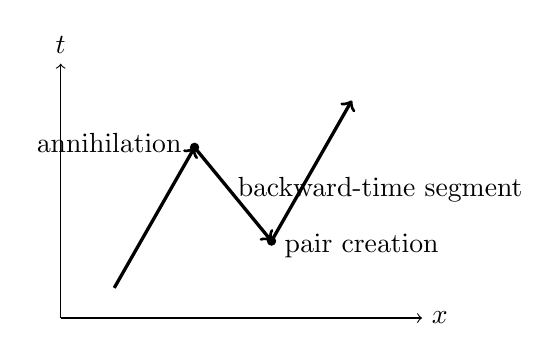
\begin{tikzpicture}[scale=0.85]
\draw[->] (0,0) -- (0,3.8) node[above] {$t$};
\draw[->] (0,0) -- (5.4,0) node[right] {$x$};
\draw[very thick,->] (0.8,0.45) -- (2.0,2.55);
\draw[very thick,->] (2.0,2.55) -- (3.15,1.15);
\draw[very thick,->] (3.15,1.15) -- (4.35,3.25);
\fill (2.0,2.55) circle (2pt);
\fill (3.15,1.15) circle (2pt);
\node[left] at (1.95,2.62) {annihilation};
\node[right] at (3.20,1.08) {pair creation};
\node[right] at (2.50,1.92) {backward-time segment};
\end{tikzpicture}
\caption{A backward-time segment read forward as pair creation and annihilation.}
\end{figure}

The factorials appearing at high orders control the exponential power series, but that is not the same as controlling the full sum over field configurations.

\begin{classroomqa}
\lecturetimestamp{01:00:00}
\audiencequestion{Do the factors of \(1/n!\) guarantee convergence?}
\lecturerresponse{They guarantee convergence of the exponential series for a fixed argument. They do not by themselves guarantee convergence of the separate sum over all field configurations. Those are distinct questions. On a finite lattice with a finite discretized set of field values the configuration count is finite, but the continuum and infinite-volume limits require further control.}
\end{classroomqa}

\section{One Link Product, Several Particle Readings}

The second-order product contains more than one-particle propagation. When its two neighboring pairs share an endpoint, it can move one particle through a two-link chain:
\begin{equation}
\bigl[\phi(x_0)\phi(x_1)\bigr]
\bigl[\phi(x_1)\phi(x_2)\bigr].
\end{equation}
When the selected pairs are separate, the same second-order term can move two particles by one link each.\footnote{The comparison between one-particle propagation and two independent one-link hops is reconstructed from the board discussion at 01:00:46--01:02:34.}
\begin{equation}
\bigl[\phi(x_0)\phi(x_1)\bigr]
\bigl[\phi(y_0)\phi(y_1)\bigr],
\qquad x_0\neq y_0.
\end{equation}
The first factor transports one particle and the second transports another. Thus the quadratic lattice expansion contains propagation amplitudes in every multiparticle sector. The same algebraic order may describe one longer connected route or several shorter disconnected routes.

This is a great deal of information, but it is not yet a genuine interaction vertex. With only quadratic propagation terms, connected particle lines do not split into a different number of lines. Particle-number-changing processes require additional interactions, even though local operator products may admit several creation-and-annihilation readings.

\begin{classroomqa}
\lecturetimestamp{01:03:30}
\audiencequestion{Could an electron and a positron annihilate and leave no particles at all?}
\lecturerresponse{A contribution with nonzero incoming energy and no energy-carrying final state violates energy conservation. When its possible spacetime positions are summed, the amplitudes cancel. Electron--positron annihilation can occur when another field carries away the energy---for example, when electromagnetic quanta are produced.}
\end{classroomqa}

\editorialnote{The abbreviated exchange moves directly from quadratic hopping to electron--positron annihilation. The secure distinction is that quadratic terms supply free propagation, while physical annihilation requires an interaction with another field; the no-output amplitude cancels by energy conservation.}

The derivative terms therefore do much, but not everything. Further terms in the Lagrangian are fixed by the experimentally observed properties and interactions of the fields.

\section{The Mass Term}

For a scalar field, the derivative structure under discussion has the schematic Lorentzian sign pattern
\begin{equation}
\mathcal{L}_{\mathrm{kin}}
\sim
\frac{1}{2}\left[
(\partial_t\phi)^2
-(\partial_x\phi)^2
-(\partial_y\phi)^2
-(\partial_z\phi)^2
\right].
\end{equation}
This display fixes the temporal-minus-spatial structure relevant to the discussion; overall signs and normalization conventions are left implicit.

The Lagrangian may also contain powers of the undifferentiated field. The quadratic example has the form
\begin{equation}
\text{mass term}\ \propto\ \frac{1}{2}m^2\phi^2,
\end{equation}
with \(m^2\) identified as the mass coefficient.\editorialnote{The source does not fix the overall sign convention for the complete scalar Lagrangian in this passage.} In the schematic particle reading, this term annihilates a particle and recreates it at the same lattice site. It does not displace the particle. It inserts a same-site factor into a path:
\begin{equation}
\text{particle at }x
\longrightarrow
\boxed{m^2\phi(x)^2}
\longrightarrow
\text{particle still at }x.
\end{equation}
Every time such an insertion acts, the path acquires another factor proportional to \(m^2\).

If only the derivative terms are retained, the resulting propagation is the massless theory in this schematic expansion. For a massive field, a route may include any number of same-site mass insertions between its hopping terms. The mass term changes the relative weights of the paths so that the resulting propagator carries the particle's mass.

\section{Cubic Terms and Split--Rejoin Histories}

The mass term changes the weight of a path without moving the particle. More interesting behavior begins with terms of degree higher than two. Take a cubic interaction,
\begin{equation}
\mathcal{L}_{\mathrm{int}}=g_3\phi^3.
\end{equation}
At one lattice cell, the three field factors have four particle readings:
\begin{equation}
1\longrightarrow 2,
\qquad
2\longrightarrow 1,
\qquad
0\longrightarrow 3,
\qquad
3\longrightarrow 0.
\end{equation}
Thus a cubic factor may annihilate one particle and create two, annihilate two and create one, create three, or annihilate three.

The quadratic neighboring-pair factors still supply propagation. A sequence of them can carry a particle to a cell, a cubic factor at that cell can absorb it and emit two particles, and further quadratic factors can carry those two particles away. This contributes to an amplitude with one incoming particle and two outgoing particles.\footnote{The lattice geometry is reconstructed from the diagram at 01:08:48--01:09:42.}

\begin{figure}[htbp]
\centering
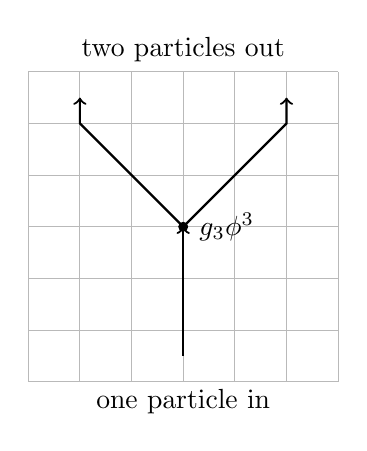
\begin{tikzpicture}[scale=0.82]
\draw[step=0.8,gray!55,thin] (0,0) grid (4.8,4.8);
\draw[thick,->] (2.4,0.4) -- (2.4,1.2) -- (2.4,2.0) -- (2.4,2.4);
\fill (2.4,2.4) circle (2.2pt);
\draw[thick,->] (2.4,2.4) -- (1.6,3.2) -- (0.8,4.0) -- (0.8,4.4);
\draw[thick,->] (2.4,2.4) -- (3.2,3.2) -- (4.0,4.0) -- (4.0,4.4);
\node[right] at (2.5,2.4) {$g_3\phi^3$};
\node at (2.4,-0.3) {one particle in};
\node at (2.4,5.15) {two particles out};
\end{tikzpicture}
\caption{Quadratic factors propagate a particle into and away from a cubic splitting vertex.}
\end{figure}

Even an amplitude with one particle both initially and finally is no longer merely a sum of single uninterrupted routes. One contribution is direct propagation by a chain of quadratic hops. Another contribution contains two cubic factors: the particle splits into two and the two later rejoin. The intermediate state may therefore contain more particles than the external state.\footnote{The two alternatives are reconstructed from the diagram at 01:09:44--01:11:36.}

\begin{figure}[htbp]
\centering
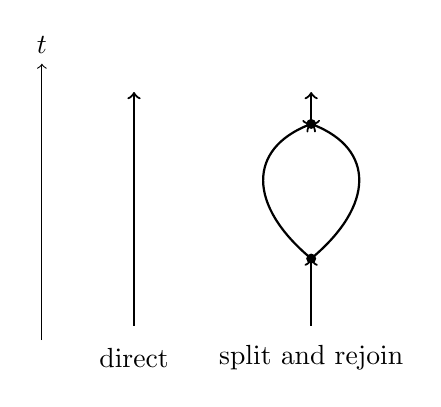
\begin{tikzpicture}[scale=0.9]
\draw[->] (-0.7,0) -- (-0.7,3.9) node[above] {$t$};
\draw[thick,->] (0.6,0.2) -- (0.6,3.5);
\node at (0.6,-0.25) {direct};
\draw[thick,->] (3.1,0.2) -- (3.1,1.15);
\fill (3.1,1.15) circle (2pt);
\draw[thick,->] (3.1,1.15) .. controls (2.2,1.9) and (2.2,2.7) .. (3.1,3.05);
\draw[thick,->] (3.1,1.15) .. controls (4.0,1.9) and (4.0,2.7) .. (3.1,3.05);
\fill (3.1,3.05) circle (2pt);
\draw[thick,->] (3.1,3.05) -- (3.1,3.5);
\node at (3.1,-0.25) {split and rejoin};
\end{tikzpicture}
\caption{Direct propagation and a split--rejoin contribution to the same one-particle amplitude.}
\end{figure}

In electrodynamics the corresponding example is an electron that emits a photon and later reabsorbs it. That emission-and-reabsorption history is part of the amplitude for the electron to propagate from one point to another. Higher orders contain several emissions and absorptions. A photon may convert into an electron--positron pair, and the electron and positron in that intermediate pair may themselves exchange a photon. Nothing requires the intermediate particle content to look simple merely because the initial and final particle content is simple.\footnote{The examples in the following reconstruction occur at 01:11:22--01:12:34.}

\begin{figure}[htbp]
\centering
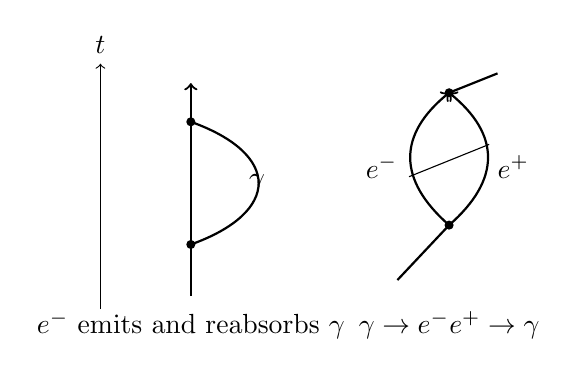
\begin{tikzpicture}[scale=0.82]
\draw[->] (-0.6,0) -- (-0.6,3.8) node[above] {$t$};
\draw[thick,->] (0.8,0.2) -- (0.8,3.5);
\fill (0.8,1.0) circle (2pt);
\fill (0.8,2.9) circle (2pt);
\draw[thick] (0.8,1.0) .. controls (2.2,1.5) and (2.2,2.4) .. (0.8,2.9);
\node[right] at (1.55,1.95) {$\gamma$};
\node at (0.8,-0.25) {$e^-$ emits and reabsorbs $\gamma$};
\draw[thick] (4.0,0.45) -- (4.8,1.3);
\fill (4.8,1.3) circle (2pt);
\draw[thick,->] (4.8,1.3) .. controls (4.0,2.0) and (4.0,2.7) .. (4.8,3.35);
\draw[thick,->] (4.8,1.3) .. controls (5.6,2.0) and (5.6,2.7) .. (4.8,3.35);
\fill (4.8,3.35) circle (2pt);
\draw[thick] (4.8,3.35) -- (5.55,3.65);
\draw[thin] (4.18,2.05) -- (5.42,2.55);
\node[left] at (4.15,2.2) {$e^-$};
\node[right] at (5.4,2.2) {$e^+$};
\node at (4.8,-0.25) {$\gamma\to e^-e^+\to\gamma$};
\end{tikzpicture}
\caption{An electron self-emission contribution and a photon history containing an electron--positron pair.}
\end{figure}

Each such history comes from a definite product of terms in the expansion of the exponential. Its coefficient carries the appropriate power of \(i\), a factorial from the exponential series, and the couplings attached to its vertices. The coefficient supplies the contribution of that history, but the amplitude for the specified initial and final states is the sum of all histories with those same external states.

\begin{classroomqa}
\lecturetimestamp{01:13:18}
\audiencequestion{Can the same overall process occur in several different histories, so that all of them contribute to its amplitude?}
\lecturerresponse{Yes. The amplitude for the process is obtained from all the different histories that join the same initial state to the same final state.}
\end{classroomqa}

There are therefore two equivalent ways to organize quantum field theory. In the field description, one specifies an initial field configuration and a final field configuration and sums over every intervening field history. In the particle description, the field is resolved into quanta: one specifies the incoming particle content and the outgoing particle content and sums all the particle histories connecting them. The same Lagrangian governs both descriptions.

\section{Quartic Terms, Conservation Laws, and Couplings}

A quartic interaction,
\begin{equation}
\mathcal{L}_{\mathrm{int}}=g_4\phi^4,
\end{equation}
has four field factors at one point. Its local particle readings include
\begin{equation}
\begin{gathered}
2\longrightarrow2,
\qquad
1\longrightarrow3,
\qquad
3\longrightarrow1,\\
0\longrightarrow4,
\qquad
4\longrightarrow0.
\end{gathered}
\end{equation}
A single four-leg vertex can therefore describe two-particle scattering, one particle splitting into three, three joining into one, or all four legs oriented outward or inward.\footnote{The orientations are reconstructed from the diagram at 01:14:28--01:15:18.}

\begin{figure}[htbp]
\centering
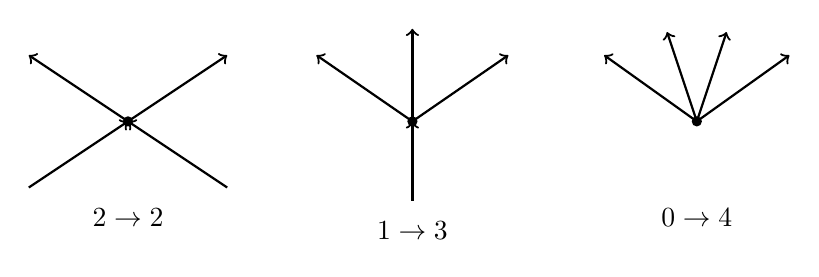
\begin{tikzpicture}[scale=0.84]
\fill (0,0) circle (2.2pt);
\draw[thick,->] (-1.5,-1.0) -- (0,0);
\draw[thick,->] (1.5,-1.0) -- (0,0);
\draw[thick,->] (0,0) -- (-1.5,1.0);
\draw[thick,->] (0,0) -- (1.5,1.0);
\node at (0,-1.45) {$2\to2$};
\begin{scope}[xshift=4.3cm]
\fill (0,0) circle (2.2pt);
\draw[thick,->] (0,-1.2) -- (0,0);
\draw[thick,->] (0,0) -- (-1.45,1.0);
\draw[thick,->] (0,0) -- (0,1.4);
\draw[thick,->] (0,0) -- (1.45,1.0);
\node at (0,-1.65) {$1\to3$};
\end{scope}
\begin{scope}[xshift=8.6cm]
\fill (0,0) circle (2.2pt);
\draw[thick,->] (0,0) -- (-1.4,1.0);
\draw[thick,->] (0,0) -- (-0.45,1.35);
\draw[thick,->] (0,0) -- (0.45,1.35);
\draw[thick,->] (0,0) -- (1.4,1.0);
\node at (0,-1.45) {$0\to4$};
\end{scope}
\end{tikzpicture}
\caption{Three local orientations of a four-leg interaction vertex.}
\end{figure}

The local reading \(0\to4\) does not by itself say that four particles can appear from the vacuum as a physical process. The vertex must still be summed over every possible spacetime position. When the proposed external state cannot conserve energy, the phases from those positions cancel.

\begin{classroomqa}
\lecturetimestamp{01:15:18}
\audiencequestion{Does the four-out orientation describe the spontaneous arrival of four particles in the final state?}
\lecturerresponse{It is one local reading of the four-field operator, but a process with no incoming energy violates energy conservation. When the amplitudes from all possible spacetime positions of the vertex are added, they cancel to zero.}
\end{classroomqa}

\begin{classroomqa}
\lecturetimestamp{01:15:58}
\audiencequestion{Do conservation of energy and conservation of momentum emerge from the calculation itself?}
\lecturerresponse{Yes. Integrating the vertex over all time enforces energy conservation, and integrating it over all space enforces momentum conservation. The sum over vertex positions vanishes unless both are conserved.}
\end{classroomqa}

Subject to those conservation laws, every graph allowed by the Lagrangian contributes some amplitude. The size of that contribution depends in part on the coefficient of each interaction term. Write the cubic and quartic coefficients as \(G_3\) and \(G_4\). Every three-leg vertex contributes one factor of \(G_3\), and every four-leg vertex contributes one factor of \(G_4\). A graph with \(V_3\) cubic vertices and \(V_4\) quartic vertices therefore has the schematic coupling dependence
\begin{equation}
\mathcal{A}_{\mathrm{graph}}
\propto G_3^{V_3}G_4^{V_4}.
\end{equation}

If these couplings are small, a graph with few vertices generally contributes more than a graph with many vertices. Each additional vertex brings another small factor. This gives the perturbative sum a chance to be useful: begin with the simplest graphs, then add successively smaller corrections.

Whether the complete series actually converges is a difficult question. Small couplings make the ordering plausible, but they do not by themselves settle every convergence problem. At large coupling the naive series may fail altogether. Such failure does not show that the underlying theory is wrong; it may show only that expansion in powers of the coupling was a poor way to calculate it. The methods under discussion are most directly useful when the couplings are small enough that a graph with four vertices is much smaller than one with two.

\begin{classroomqa}
\lecturetimestamp{01:19:24}
\audiencequestion{Can color theory be treated in the same way?}
\lecturerresponse{Yes. Color theory can be formulated in the same way and will be discussed later.}
\end{classroomqa}

\section{Propagators, Vertices, and Complementary Descriptions}

The next task is to list the particles and encode their dynamics either in a Lagrangian or in Feynman rules. These are two forms of the same information. Quadratic terms describe propagation from one point to another. A line representing that propagation is called a propagator. Terms involving three or more fields describe places where lines meet. Those meeting points are vertices. For example,
\begin{equation}
\begin{aligned}
\text{quadratic term}
&\longleftrightarrow \text{propagator},\\
G_3\phi^3
&\longleftrightarrow \text{three-leg vertex}.
\end{aligned}
\end{equation}

One can specify a theory by giving a quantum field for every particle and writing one Lagrangian containing all their masses and interactions. Equivalently, one can list every propagator, every allowed vertex, and the coefficient attached to each vertex. Either list tells us what processes are possible and how to assign amplitudes to their graphs.

For example, two electrons can scatter by exchanging a photon. Each electron line contains an electron--electron--photon vertex, and the photon propagator joins the two vertices.\footnote{The diagram is reconstructed from the example at 01:21:38.}

\begin{figure}[htbp]
\centering
\begin{tikzpicture}[scale=0.95]
\draw[->] (-0.6,-0.2) -- (0.2,1.4);
\draw[->] (0.2,1.4) -- (-0.7,3.1);
\draw[->] (3.5,-0.2) -- (2.7,1.4);
\draw[->] (2.7,1.4) -- (3.6,3.1);
\fill (0.2,1.4) circle (2pt);
\fill (2.7,1.4) circle (2pt);
\draw[thick] (0.2,1.4) -- (2.7,1.4);
\node[above] at (1.45,1.4) {$\gamma$};
\node[left] at (-0.2,0.5) {$e^-$};
\node[right] at (3.1,0.5) {$e^-$};
\end{tikzpicture}
\caption{Two-electron scattering through the exchange of a photon.}
\end{figure}

The Lagrangian determines the amplitude for this graph and contains the symmetries and conservation laws that constrain it. In a time-oriented drawing, particles placed at the bottom form the initial configuration and particles at the top form the final configuration.

\begin{classroomqa}
\lecturetimestamp{01:22:06}
\audiencequestion{In a Feynman diagram, are the particles at the bottom the initial configuration and those at the top the final configuration?}
\lecturerresponse{Yes. The bottom is the initial particle configuration, and the top is the final particle configuration.}
\end{classroomqa}

The particle description and the field description are complementary, much as momentum and position are complementary descriptions in ordinary quantum mechanics. They describe the same system in different bases. There is also a corresponding uncertainty: if particle number is specified precisely, the field value is uncertain; if the field value is specified precisely, particle number is uncertain. Neither description replaces the other, and the Lagrangian is useful in both.

\begin{classroomqa}
\lecturetimestamp{01:23:26}
\audiencequestion{Are the coupling constants predicted by theory, or are they determined experimentally?}
\lecturerresponse{Symmetries can sometimes relate one coupling constant to another, but their numerical values generally come from experiment.}
\end{classroomqa}

\section{Measured Inputs and Broad Predictions}

Quantum field theory itself has elegance and beauty. But when one starts listing the facts---what particles there are, what their masses are, and what their coupling constants are---the list is a mess. It is a very ugly mess, with very little coherence except the coherence supplied by symmetries. Symmetries relate different kinds of particles and their processes, but only to a limited extent. Much of the inventory remains a large collection of comparatively random facts about a somewhat unmotivated collection of different kinds of particles.

\begin{classroomqa}
\lecturetimestamp{01:24:58}
\audiencequestion{Why should the measured coupling constants be trusted so confidently?}
\lecturerresponse{Once a coupling has been measured, changing it gives incorrect predictions. Its value is tested by the many calculations that use it.}
\end{classroomqa}

There are too many particles, which means too many fields---too many for any aesthetic sense. There are roughly a hundred or so. There are many coupling constants, more or less numbers pulled from experiment, and many masses, which range all over the map. There are a few relations among them, but only a few.

But once you know them, you can start to calculate. Once you know them, that is it: one can calculate with great precision anything about those particles. Anything about quarks, electrons, photons, and the rest reaches into atomic physics, particle physics, nuclear physics, chemistry, and perhaps biology. The amount of input may be larger than one would like, but the amount of output is huge.

\section{Quantum Electrodynamics as a Perturbative Example}

Quantum electrodynamics gives a concrete example of the coupling expansion.

\begin{classroomqa}
\lecturetimestamp{01:26:12}
\audiencequestion{For electrons and photons, how many interaction couplings of the \(G_n\) type are there?}
\lecturerresponse{There is one elementary interaction coupling: the electric charge \(e\). It is a \(G_3\)-type coefficient attached to a vertex with an electron entering, an electron leaving, and a photon emitted or absorbed.}
\end{classroomqa}

Suppressing the spinor matrices and indices, the interaction has the schematic field content
\begin{equation}
\mathcal{L}_{\mathrm{QED,int}}
\sim e\,(\text{electron bilinear})\,A,
\end{equation}
where \(A\) denotes the photon field. The detailed Dirac-matrix structure is not needed for the counting argument. The elementary QED rule is the emission or absorption of a photon by an electron; all the more complicated QED graphs are assembled from repeated uses of that one vertex.\footnote{The schematic vertex is reconstructed from 01:26:42; the detailed matrix structure is deliberately suppressed in the source.}

\begin{figure}[htbp]
\centering
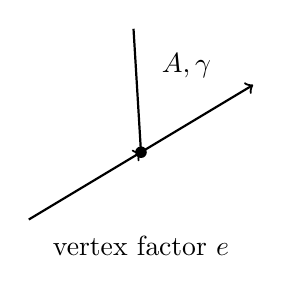
\begin{tikzpicture}[scale=0.95]
\draw[thick,->] (-1.5,-0.9) -- (0,0);
\draw[thick,->] (0,0) -- (1.5,0.9);
\draw[thick] (0,0) -- (-0.1,1.65);
\fill (0,0) circle (2.2pt);
\node[right] at (0.15,1.15) {$A,\gamma$};
\node at (0,-1.25) {vertex factor $e$};
\end{tikzpicture}
\caption{The elementary electron--electron--photon vertex of quantum electrodynamics.}
\end{figure}

\begin{classroomqa}
\lecturetimestamp{01:27:38}
\audiencequestion{What about electron--proton scattering?}
\lecturerresponse{In the elementary atomic treatment, the proton can be idealized as a fixed, infinitely heavy point source---a heavy particle nailed down in place. Its own quantum-field dynamics enter only when the internal theory of protons and neutrons is included.}
\end{classroomqa}

\begin{classroomqa}
\lecturetimestamp{01:28:30}
\audiencequestion{Can the electron move nearly at the speed of light relative to that proton?}
\lecturerresponse{Yes.}
\end{classroomqa}

Consider photon scattering by an electron. At lowest order the graph has two electron--electron--photon vertices. The amplitude is therefore proportional to \(e^2\):
\begin{equation}
\mathcal{A}_{\mathrm{lowest}}\propto e^2.
\end{equation}
The probability, or equivalently the coupling dependence of the cross section, comes from the absolute square and is proportional to \(e^4\):
\begin{equation}
P_{\mathrm{lowest}}\ \text{or}\ \sigma_{\mathrm{lowest}}
\propto e^4.
\end{equation}
With the conventional dimensionless normalization, the electric coupling is small, so genuine scattering is much less likely than the photon simply passing without scattering.

There are already two graphs at this order. In one ordering the incoming photon is absorbed and the outgoing photon is emitted later. In the other, the outgoing photon is emitted before the incoming photon is absorbed. Both amplitudes contribute.\footnote{The two time orderings are reconstructed from the diagrams at 01:28:42 and 01:30:18.}

\begin{figure}[htbp]
\centering
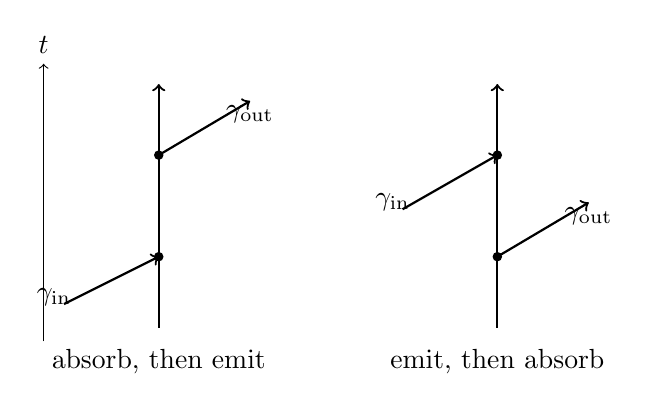
\begin{tikzpicture}[scale=0.86]
\draw[->] (-0.7,0) -- (-0.7,4.1) node[above] {$t$};
\draw[thick,->] (1.0,0.2) -- (1.0,3.8);
\fill (1.0,1.25) circle (2pt);
\fill (1.0,2.75) circle (2pt);
\draw[thick,->] (-0.4,0.55) -- (1.0,1.25);
\draw[thick,->] (1.0,2.75) -- (2.35,3.55);
\node[left] at (-0.15,0.65) {$\gamma_{\mathrm{in}}$};
\node[right] at (1.85,3.35) {$\gamma_{\mathrm{out}}$};
\node at (1.0,-0.3) {absorb, then emit};
\begin{scope}[xshift=5.0cm]
\draw[thick,->] (1.0,0.2) -- (1.0,3.8);
\fill (1.0,1.25) circle (2pt);
\fill (1.0,2.75) circle (2pt);
\draw[thick,->] (1.0,1.25) -- (2.35,2.05);
\draw[thick,->] (-0.4,1.95) -- (1.0,2.75);
\node[right] at (1.85,1.85) {$\gamma_{\mathrm{out}}$};
\node[left] at (-0.15,2.05) {$\gamma_{\mathrm{in}}$};
\node at (1.0,-0.3) {emit, then absorb};
\end{scope}
\end{tikzpicture}
\caption{The two lowest-order time orderings for electron--photon scattering.}
\end{figure}

The lowest-order amplitude is consequently not one graph but the sum of the two:
\begin{equation}
\begin{aligned}
\mathcal{A}^{(2)}
&=
\mathcal{A}_{\mathrm{absorb\ then\ emit}}
+\mathcal{A}_{\mathrm{emit\ then\ absorb}},\\
\mathcal{A}^{(2)}&\propto e^2.
\end{aligned}
\end{equation}

Higher-order corrections add more elementary vertices. An additional internal photon attached twice to the electron line adds two factors of \(e\), giving a contribution proportional to \(e^4\) in the amplitude and \(e^8\) in its squared magnitude. A photon line may also contain an electron--positron insertion, again adding elementary vertices and additional powers of \(e\). These are examples, not an exhaustive list; the extra photon can be attached in many positions.\footnote{The higher-order structures are reconstructed from 01:30:38--01:31:16.}

\begin{figure}[htbp]
\centering
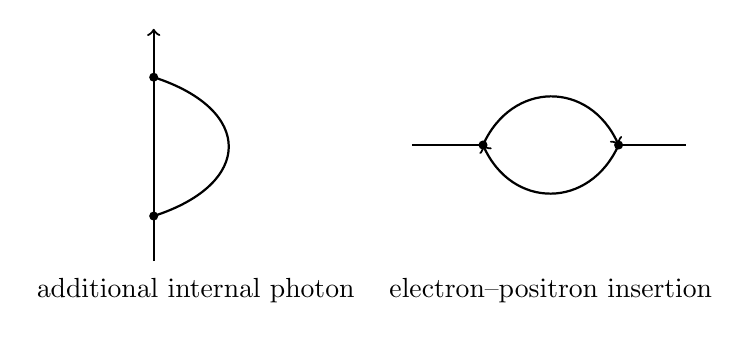
\begin{tikzpicture}[scale=0.82]
\draw[thick,->] (0.9,0.2) -- (0.9,3.8);
\fill (0.9,0.9) circle (2pt);
\fill (0.9,3.05) circle (2pt);
\draw[thick] (0.9,0.9) .. controls (2.45,1.4) and (2.45,2.55) .. (0.9,3.05);
\node at (1.55,-0.25) {additional internal photon};
\begin{scope}[xshift=5.1cm]
\draw[thick] (-0.2,2.0) -- (0.9,2.0);
\fill (0.9,2.0) circle (2pt);
\fill (3.0,2.0) circle (2pt);
\draw[thick,->] (0.9,2.0) .. controls (1.35,3.0) and (2.55,3.0) .. (3.0,2.0);
\draw[thick,->] (3.0,2.0) .. controls (2.55,1.0) and (1.35,1.0) .. (0.9,2.0);
\draw[thick] (3.0,2.0) -- (4.05,2.0);
\node at (1.95,-0.25) {electron--positron insertion};
\end{scope}
\end{tikzpicture}
\caption{Two higher-order QED structures that add elementary vertices and further powers of \(e\).}
\end{figure}

Thus the QED expansion proceeds in successive powers of \(e^2\). Each comparable new complication adds two powers of the electric charge to the amplitude. In the normalization being used, that makes such a correction roughly a hundred or a couple of hundred times smaller in amplitude than the preceding order. The more complicated graphs are progressively weaker, so the perturbative sum has a chance to be useful.

The probability is not obtained by squaring each graph separately and then adding those squares. First add every amplitude contributing to the same external process:
\begin{equation}
\mathcal{A}_{\mathrm{total}}=\sum_r\mathcal{A}_r.
\end{equation}
Only then form
\begin{equation}
P=\left|\mathcal{A}_{\mathrm{total}}\right|^2
=\left|\sum_r\mathcal{A}_r\right|^2.
\end{equation}
The cross terms between different graphs are interference terms. The rule is simple and essential: add first, then square.

\section{Toward the Particle Inventory and the Standard Model}

With propagators, vertices, coupling counting, and interference in place, the particle-physics description can begin in earnest. One can name the particles, specify their masses, write the Lagrangians that govern them partly from theory and partly from experiment, and study their symmetries directly in those Lagrangians. The same framework then leads to the Standard Model and its properties.

\begin{classroomqa}
\lecturetimestamp{01:33:22}
\audiencequestion{Could the constant mass coefficient \(m^2\) be replaced by the Higgs field?}
\lecturerresponse{Yes. That is the right idea, and the mechanism will be discussed later.}
\end{classroomqa}

\begin{classroomqa}
\lecturetimestamp{01:33:42}
\audiencequestion{Can the neighboring lattice points \(x\) and \(x'\) lie at two different times?}
\lecturerresponse{Yes. They may be neighbors in the time direction; that is how vertical propagation on the lattice is represented.}
\end{classroomqa}

For neighboring points, the finite-difference square contains both same-site and cross-link terms:
\begin{equation}
\bigl[\phi(x)-\phi(x')\bigr]^2
=
\phi(x)^2+\phi(x')^2-2\phi(x)\phi(x').
\end{equation}

\begin{classroomqa}
\lecturetimestamp{01:33:56}
\audiencequestion{Which term represents a particle simply standing still?}
\lecturerresponse{The same-site terms \(\phi(x)^2\) and \(\phi(x')^2\) in the finite-difference square represent standing still, while the cross term \(\phi(x)\phi(x')\) supplies the moving interpretation. The explicit mass term also contributes same-site, standing-still factors.}
\end{classroomqa}
